\chapter{Исследовательская часть}

\section{Замеры количества сравнений}

Замеры проводились на массивах длины 1091. Каждый элемент массива во время замеров равен его индексу. Во время замеров для каждого элемента в массиве вызывался его поиск. Также был поиск элемента, отсутствующего в массиве. При установке в переменную returnsComprasionCount значения true все функции возвращают число сравнений вместо результата. Результаты представлены на рисунках \ref{fig:res1}, \ref{fig:res2} и \ref{fig:res1}.

\begin{figure}[h!]
	\centering
	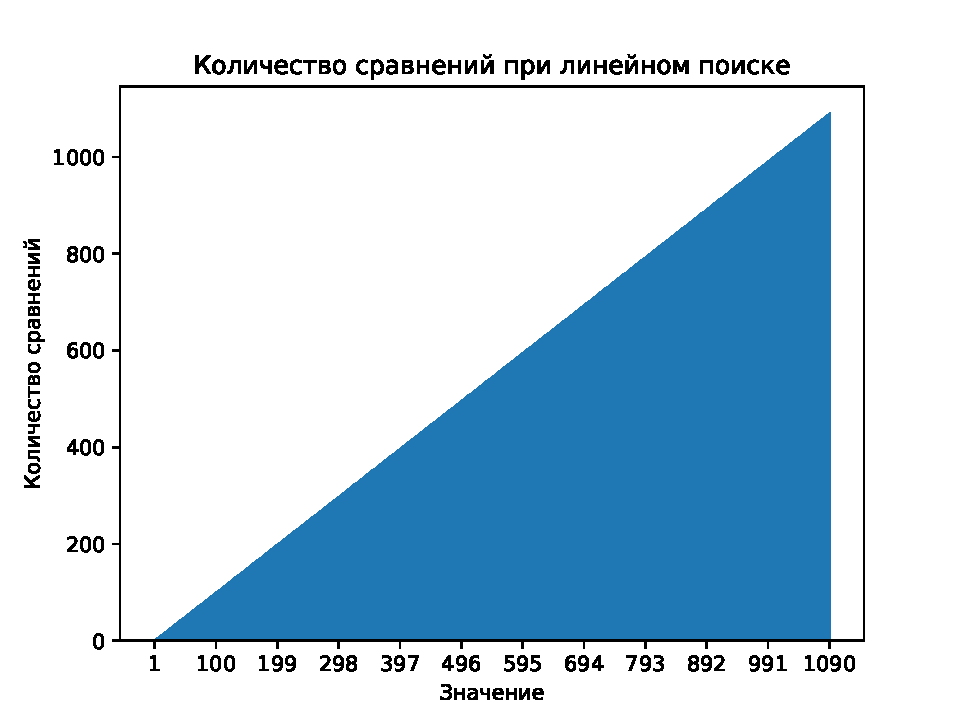
\includegraphics[width=1\textwidth]{tex_parts/linear_graph.pdf}
	\caption{\label{fig:res1} Результаты замера числа сравнений для алгоритма линейного поиска}
\end{figure}

\clearpage

\begin{figure}[h!]
	\centering
	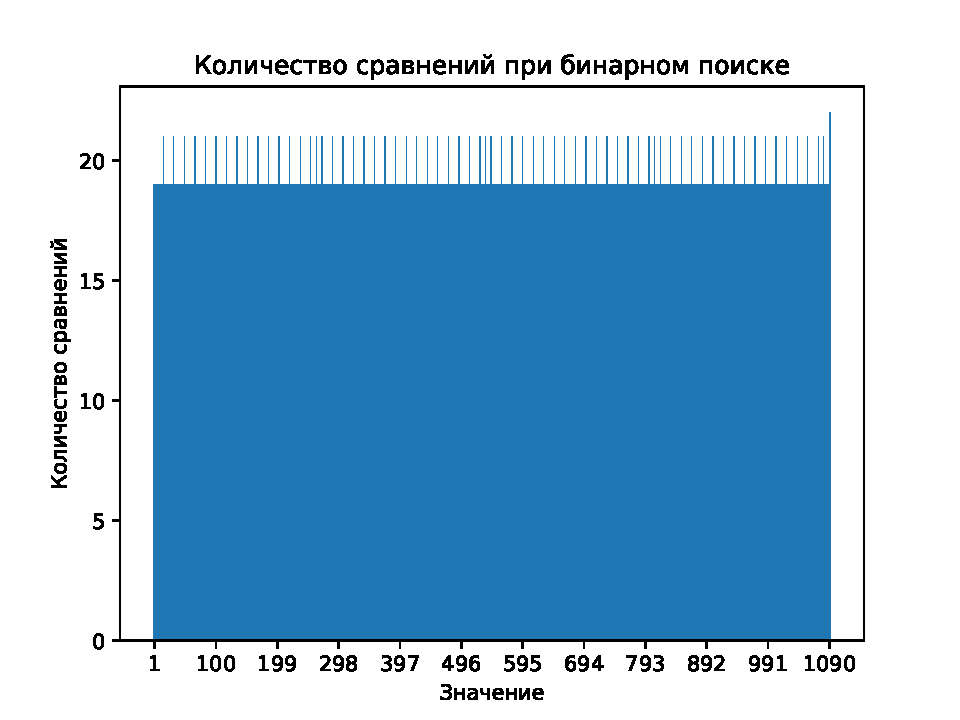
\includegraphics[width=0.8\textwidth]{tex_parts/binary_graph.pdf}
	\caption{\label{fig:res2} Результаты замера числа сравнений для алгоритма бинарного поиска}
\end{figure}

\begin{figure}[h!]
	\centering
	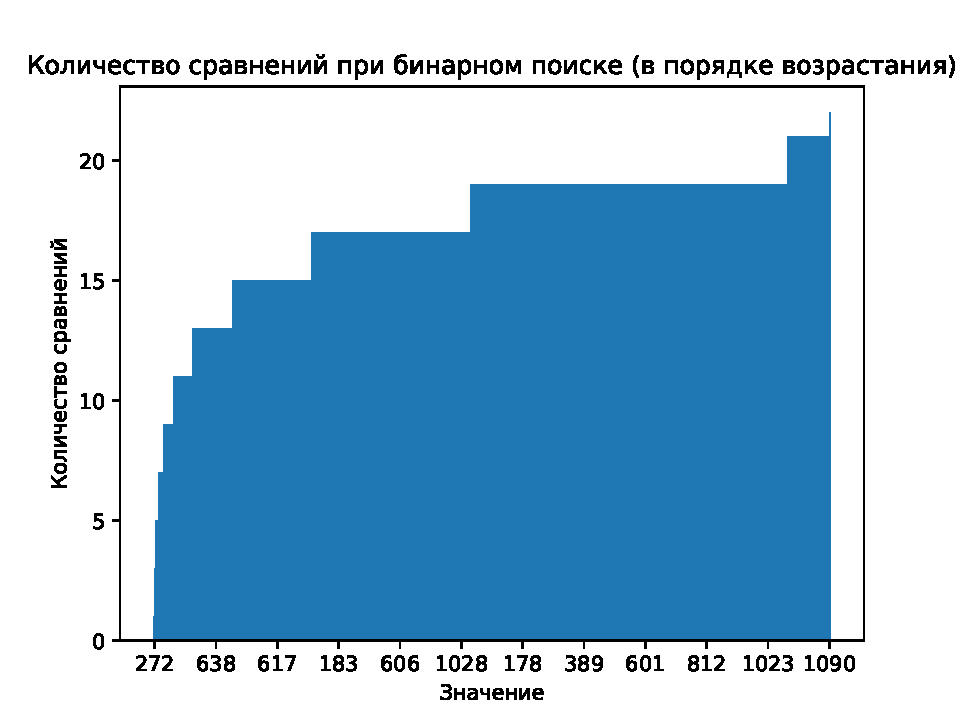
\includegraphics[width=0.8\textwidth]{tex_parts/sorted_graph.pdf}
	\caption{\label{fig:res3} Отсортированные результаты замера числа сравнений для алгоритма бинарного поиска}
\end{figure}

\clearpage

Результаты совпали с расчетами, алгоритм линейного поиска в худшем случае сделал больше 1000 сравнений, в то время как алгоритм бинарного поиска сделал меньше 25 сравнений.

\section{Вывод}

В данном разделе были проведены замеры числа сравнений. Алгоритм бинарного поиска оказался эффективнее алгоритма линейного поиска по числу сравнений. 
